% MLR570 survey -- TMLR template (vendored in tmlr/, Apache-2.0, upstream 7bf90ef).
% Build:  cd paper/survey && latexmk     (settings in latexmkrc; output in build/)
\documentclass[10pt]{article}
\usepackage[preprint]{tmlr}   % [preprint] shows author names
\usepackage[utf8]{inputenc}
\usepackage[T1]{fontenc}
\usepackage{amsmath,amssymb,amsfonts}
\usepackage{booktabs,multirow,graphicx,xcolor,array}
\usepackage{tikz}
\usepackage{hyperref}
\usepackage{url}

\title{State-of-the-Art Knowledge Distillation: A Survey of Knowledge Types,
Training Schemes, and Multi-Objective Optimization}

\author{\name Khalid Hamdan \email TBD \\ \addr American University of Sharjah
  \AND \name Aly Khaled Ismail Mahmoud \email TBD \\ \addr American University of Sharjah
  \AND \name Hasan Akel \email TBD \\ \addr American University of Sharjah
  \AND \name Salim Akel \email TBD \\ \addr American University of Sharjah}

\def\month{MM}
\def\year{2026}
\def\openreview{\url{https://openreview.net/forum?id=XXXX}}

\begin{document}
\maketitle

\begin{abstract}
\textit{[To be written last (Task 15): motivation, key contributions, high-level structure, key trends (G2).]}
\end{abstract}

% Owner: Khalid  |  Task: T4, T15  |  Drafted by ORCA agents, finalised by the owner.
% Rules: prose only; every claim cited with \citet/\citep to a literature/sources.yaml record id;
% compare methods (G6); strengths/weaknesses/applicability (G8). See tasks/todo.md.
\section{Introduction}
\label{sec:intro}
\textit{[To be written: Problem statement and trends; motivation and gap; Table I (comparison with existing surveys); Fig. 1 taxonomy; scope; organisation.]}

% Owner: Aly  |  Task: T5  |  Drafted by ORCA agents, finalised by the owner.
% Rules: prose only; every claim cited with \citet/\citep to a literature/sources.yaml record id;
% compare methods (G6); strengths/weaknesses/applicability (G8). See tasks/todo.md.
\section{Preliminaries}
\label{sec:prelim}
\textit{[To be written: Notation; Hinton KD (CE + $T^2$ KL); temperature; benchmarks and teacher--student pairs; Fig. 2 KD pipeline.]}

% Owner: Aly  |  Task: T6  |  Drafted by ORCA agents, finalised by the owner.
% Rules: prose only; every claim cited with \citet/\citep to a literature/sources.yaml record id;
% compare methods (G6); strengths/weaknesses/applicability (G8). See tasks/todo.md.
% All numbers: CIFAR-100 top-1 (%), ResNet32x4 -> ResNet8x4 unless stated; each paper's own claim,
% read from the primary PDF on 2026-11-07 (table given in a "% src:" comment next to each number).
% Condensed 2026-11-08 (tasks/condense.md); full text at git tag survey-full-v1.
\section{Logit-Based Distillation}
\label{sec:logit}

Logit-based methods supervise the student through the teacher's output layer. In their usual output-only form they need no projector, cost little more than training the student alone, and fit any pair of classifiers with the same label space; SDD and WKD-L are exceptions that read final or intermediate features while keeping a logit-level loss. Until 2022 they trailed feature methods: on ResNet32$\times$4$\to$ResNet8$\times$4, classical KD \citep{hinton2015kd} reaches 73.33\% against 75.51\% for CRD and 75.63\% for ReviewKD \citep[Table~6]{zhao2022dkd}.
% src: DKD Table 6 (KD 73.33, CRD 75.51, ReviewKD 75.63)
Later work closed the gap by changing what the KL term of Eq.~\eqref{eq:kd-objective} measures. We group methods by how they decompose the loss (\S\ref{sec:logit-decouple}), rescale the logits (\S\ref{sec:logit-scale}), or replace the divergence (\S\ref{sec:logit-div}); Table~\ref{tab:logit-sota} gives each method's own number on the common pair.

\subsection{Decoupling the KD loss}
\label{sec:logit-decouple}

DKD \citep{zhao2022dkd} splits KL into a binary target-class term (TCKD) and a non-target term (NCKD). In classical KD the non-target term is scaled by $1-p^{T}_{y}(\mathbf{z}_t)$ and so vanishes on the confidently predicted samples that DKD's ablation finds most useful; DKD removes this coupling with separate weights, $\alpha\,\mathrm{TCKD}+\beta\,\mathrm{NCKD}$, and lifts ResNet8$\times$4 from 73.33\% to 76.32\%, above CRD and ReviewKD at the cost of plain KD \citep[Table~6]{zhao2022dkd}. Its code base (\texttt{mdistiller}) underlies most later logit work. The authors state its limits: $\beta$ must be tuned per pair, and a logit-only loss cannot transfer the localisation knowledge detectors need, so DKD trails ReviewKD on COCO.
% src: DKD Table 6 (DKD 76.32, KD 73.33)
NKD \citep{yang2023nkd} instead normalises the non-target distributions, replacing the tuned $\beta$ with a fixed rule (76.35\%, ImageNet ResNet34$\to$ResNet18 71.96\%, \citealp[Table~1]{yang2023nkd}); the 0.03-point gap to DKD is far below the cross-paper spread of \S\ref{sec:prelim-benchmarks}. SDD \citep{wei2024sdd} decouples along space, splitting multi-scale local logits into consistent and complementary terms; SD-KD reports 76.63\% \citep[Table~6]{wei2024sdd}, but reproductions give 75.92\% \citep{xiang2025ekd} and 75.09\% \citep{xu2025ldrld}. LDRLD \citep{xu2025ldrld} distils dense relations between local class pairs (77.20\%, \citealp[Table~1]{xu2025ldrld}), at a cost that grows with the number of pairs.
% src: NKD Table 1; SDD Table 6, EKD Table 1 (75.92), LDRLD Table 1 (75.09, 77.20)
GDKD \citep{zheng2025gdkd} generalises the target/non-target split into a partition between the teacher's top classes and the rest, reporting 77.76\% against 76.64\% for its own DKD run \citep[Table~I]{zheng2025gdkd}, a baseline 0.32 points above DKD's figure. TopKD \citep{wang2025topkd} and Sort-KD \citep{limantoro2025sortkd} also move the split or reorder the teacher's logits, and LTKD \citep{kim2026ltkd} decouples by class-frequency group for long-tailed data (CIFAR-100-LT $\gamma{=}100$: 51.08\% overall and 27.21\% on tail classes against 46.11\% and 13.25\% for DKD, \citealp[Table~1]{kim2026ltkd}).
% src: GDKD T I (77.76; own DKD 76.64); LTKD Table 1. GDKD, TopKD, Sort-KD: CORE-P preprints.

\subsection{Rescaling the logits: temperature and standardisation}
\label{sec:logit-scale}

CTKD \citep{li2023ctkd} learns the temperature adversarially through a gradient-reversal layer on a curriculum; gains are modest but consistent (ImageNet KD 70.83\%$\to$71.32\%, DKD 71.13\%$\to$71.51\%, \citealp[Table~4]{li2023ctkd}), and LSKD's reproduction gives KD+CTKD 73.39\% on our pair \citep[Table~2]{sun2024lskd}. CTKD still shares one $T$ between teacher and student. LSKD \citep{sun2024lskd} argues that a small student need not reach the teacher's logit range, since only relations between logits matter, and z-score standardises each logit vector before the softmax, a per-sample temperature. As a plug-in it lifts KD from 73.33\% to 76.62\%, DKD to 77.01\% and MLKD from 77.08\% to 78.28\% \citep[Table~2]{sun2024lskd}, so standardisation and decoupling combine; gains shrink on other pairs (0.13 points for DKD on VGG13$\to$VGG8) and LDRLD reproduces KD+LS at 76.16\% \citep[Table~1]{xu2025ldrld}.
% src: CTKD Table 4; LSKD Table 2 (73.39, 76.62, 77.01, 78.28, +0.13); LDRLD Table 1 (76.16)
LumiNet \citep{hossain2025luminet} normalises each class logit with batch statistics instead, reporting 77.50\% over five runs and an expected calibration error of 0.06 against 0.11 for KD \citep[Tables~1 and~5]{hossain2025luminet}; its targets therefore depend on batch composition (INTERPRETATION). WTTM \citep{zheng2024wttm} applies the temperature to the teacher only, which equals KD plus a R\'enyi-entropy regulariser, and weights samples by the teacher's power sum (76.06\%, ImageNet 72.19\%, \citealp[Tables~2 and~5]{zheng2024wttm}). DTS \citep{islam2025dts} schedules $T$ from the teacher--student loss gap, but its MLKD baseline sits about two points below MLKD's own figure, so its gain is hard to place.
% src: LumiNet T1/T5; WTTM T2/T5; DTS T II. DTS: CORE-P.

\subsection{Replacing or enriching the KL divergence}
\label{sec:logit-div}

DIST \citep{huang2022dist} targets the capacity gap by replacing KL with inter- and intra-class Pearson correlation, which keeps the ranking of predictions while ignoring shift and scale (76.31\%, ImageNet 72.07\%, \citealp[Tables~5 and~2]{huang2022dist}); it is weaker for binary tasks. MLKD \citep{jin2023mlkd} aligns predictions at instance, batch and class level and augments them over several temperatures, reporting 77.08\% \citep[Table~2]{jin2023mlkd}; part of its gain may come from the temperature augmentation (HYPOTHESIS). WKD-L \citep{lv2024wkd} uses a discrete Wasserstein distance whose cost encodes category relations (76.53\%, 77.28\% with WKD-F, ImageNet 72.49\%, \citealp[Tables~11 and~4]{lv2024wkd}) at higher training cost, and EKD \citep{xiang2025ekd} distils a Dirichlet over class probabilities (77.21\%; 72.54\% on ImageNet ResNet50$\to$MobileNet), apparently needing an evidentially trained teacher.
% src: DIST T5/T2; MLKD T2; WKD T11/T4; EKD T1/T3
Other papers keep a KL-type loss but change its parts: DKL and its journal form GKL \citep{cui2024dkl,cui2026gkl} decompose and symmetrise KL (76.59\% and 76.83\%), BDD \citep{qi2025bdd} adds reverse KL on low-probability classes, ABKD \citep{wang2025abkd} uses an $\alpha$-$\beta$-divergence, RCKD \citep{wang2026rckd} a cosine-type loss, and GenDD \citep{cui2025gendd} a conditional generative target (77.47\%). Ranking losses form a related group: PLD \citep{bassam2025pld} folds label and teacher into one Plackett--Luce target and so needs no KD weight (authors' claim; no number extracted), the Kendall-$\tau$ term \citep{guan2025rankingkd} adds an order constraint to KL, and AR-KD \citep{jiang2026arkd} learns class correlations reciprocally.
% src: DKL T13; GKL T17; GenDD T5. Other values in tab:logit-sota or the appendix.

Batch and sample structure is the last axis. SKD \citep{jeong2026skd} adds batch Gram-matrix alignment to instance KL and reports 78.33\%, the highest single-method logit number we found, though its KD baseline of 74.75\% is about 1.4 points above the usual 73.33\% \citep[Table~1]{jeong2026skd}; IKD \citep{wang2025ikd} is a debiased batch-consistency plug-in. EA-KD \citep{su2025eakd} weights samples by entropy, 75.46\% alone and 78.38\% stacked as EA-MLD+LS \citep[Table~2]{su2025eakd}; IPWD \citep{niu2022ipwd}, TGeo-KD \citep{hu2024tgeokd} and ADG-KD \citep{li2025adgkd} weight samples by propensity, geometry or learned factors, and e$^2$KD \citep{parchami2024e2kd} adds explanation-map similarity, matching KD at full ImageNet data. RLD \citep{sun2025rld} uses the label to mask every class the teacher ranks at or above the true class, so a wrong teacher ranking is not transferred (76.64\%, 0.32 above DKD, \citealp[Table~1]{sun2025rld}); it and TGeo-KD and EA-KD are analysed further in \S\ref{sec:reliability}.
% src: SKD T1 (78.33; KD 74.75); EA-KD T2 (75.46; 78.38); RLD T1 (76.64; DKD 76.32)

\subsection{Comparison and outlook}
\label{sec:logit-compare}

% INTERPRETATION below unless cited.
Because LSKD improves KD, DKD and MLKD \citep[Table~2]{sun2024lskd} and SDD wraps KD, DKD and NKD \citep{wei2024sdd}, decomposition, rescaling and divergence behave as separable axes. The 2024--2025 methods report 76.0--77.5\%, a range comparable to cross-paper reproduction spread (\S\ref{sec:prelim-benchmarks}), so Table~\ref{tab:logit-sota} names no single best method; only the step of about three points from KD to the 2022 methods is consistent across sources. DKD and KD+LSKD are cheap baselines with public code that other papers re-report \citep[Table~1]{xiang2025ekd,xu2025ldrld}; MLKD+LSKD, SKD and EA-MLD+LS report the highest values, but with extra terms, a stronger baseline, or stacking, and most 2024--2026 plug-ins report their best numbers on top of MLKD or NKD. Recent work shifts to which teacher signal to trust (RLD; \S\ref{sec:reliability}), class imbalance (LTKD), and balancing the KD term against the task loss (PLD; \S\ref{sec:kd_moo}). \S\ref{sec:benchmarks} and the appendix list the full included set.

\begin{table}[t]
\centering
\caption{Logit-based distillation methods (NIPS-W: NIPS 2014 Deep Learning Workshop; arXiv 2015). Accuracy is CIFAR-100 top-1 (\%) for
ResNet32$\times$4$\to$ResNet8$\times$4 as given in the source table named in each cell (the method's own paper unless another paper is named, which marks a reproduction); teacher 79.42, student 72.50. Numbers come from different papers and are not a leaderboard
(\S\ref{sec:prelim-benchmarks}). n/r: not reported by the paper.}
\label{tab:logit-sota}
\footnotesize
\setlength{\tabcolsep}{3pt}
\begin{tabular}{@{}l l p{4.0cm} p{2.5cm} p{3.3cm}@{}}
\toprule
Method & Venue & Key idea & R32$\times$4$\to$R8$\times$4 & Code \\
\midrule
KD \citep{hinton2015kd} & NIPS-W 2014 & Temperature-softened teacher targets & 73.33 (DKD T6) & -- \\
DKD \citep{zhao2022dkd} & CVPR 2022 & Target / non-target terms with separate weights & 76.32 (T6) & megvii-research/mdistiller \\
DIST \citep{huang2022dist} & NeurIPS 2022 & Inter- and intra-class Pearson correlation instead of KL & 76.31 (T5) & hunto/DIST\_KD \\
CTKD \citep{li2023ctkd} & AAAI 2023 & Adversarially learned temperature on a curriculum & n/r; KD+CTKD 73.39 (LSKD T2) & zhengli97/CTKD \\
MLKD \citep{jin2023mlkd} & CVPR 2023 & Instance-, batch- and class-level alignment; multi-temperature & 77.08 (T2) & Jin-Ying/Multi-Level-Logit-Distillation \\
NKD \citep{yang2023nkd} & ICCV 2023 & Normalised non-target distributions & 76.35 (T1) & yzd-v/cls\_KD \\
WTTM \citep{zheng2024wttm} & ICLR 2024 & Teacher-only temperature; sample weights from power sum & 76.06 (T2) & zkxufo/TTM \\
LSKD \citep{sun2024lskd} & CVPR 2024 & Z-score standardised logits (plug-in) & KD+LS 76.62; MLKD+LS 78.28 (T2) & sunshangquan/logit-standardization-KD \\
SDD \citep{wei2024sdd} & CVPR 2024 & Multi-scale local logits, consistent vs complementary & SD-KD 76.63 (T6, ablation) & shicaiwei123/SDD-CVPR2024 \\
WKD \citep{lv2024wkd} & NeurIPS 2024 & Discrete Wasserstein distance over class relations & WKD-L 76.53 (T11) & JiamingLv/WKD \\
LumiNet \citep{hossain2025luminet} & TMLR 2025 & Logits normalised by intra-batch class statistics & 77.50 (T1) & ismail31416/LumiNet \\
RLD \citep{sun2025rld} & ICCV 2025 & Label-refined sample confidence and masked correlation & 76.64 (T1) & zju-SWJ/RLD \\
LDRLD \citep{xu2025ldrld} & ICCV 2025 & Dense pairwise relations between local class pairs & 77.20 (T1) & yema-web/LDRLD \\
EKD \citep{xiang2025ekd} & ICCV 2025 & Distils a Dirichlet (second-order) distribution & 77.21 (T1) & Liangyu-Xiang/EKD \\
LTKD \citep{kim2026ltkd} & CVPR 2026 & Cross-group and within-group KL, rebalanced for long-tailed data & n/r (long-tailed only; CIFAR-100-LT $\gamma{=}100$: 51.08, T1) & none found \\
DKL \citep{cui2024dkl} & NeurIPS 2024 & KL as weighted MSE + soft-label CE, symmetrised & 76.59 (T13) & jiequancui/DKL \\
Kendall-$\tau$ \citep{guan2025rankingkd} & ICML 2025 & Plug-in logit-order ranking loss & MLKD+rank 77.25 (T2) & OvernighTea/ RankingLoss-KD \\
ADG-KD \citep{li2025adgkd} & AAAI 2025 & Teacher and instance guidance fused by learned factors & 77.44; MLKD+ADG 77.51 (T1) & none found \\
SKD \citep{jeong2026skd} & CVPR 2026 & Instance KL + batch Gram-matrix alignment & 78.33 (T1; its KD 74.75) & none found \\
PLD \citep{bassam2025pld} & NeurIPS 2025 & Plackett--Luce list-wise ranking loss, no KD weight & not extracted & none found \\
\bottomrule
\end{tabular}
% src (each row checked against the primary PDF, 2026-11-07): DKD T6; DIST T5; LSKD T2 (CTKD row);
% MLKD T2; NKD T1; WTTM T2; LSKD T2; SDD T6 (Fusion); WKD T11 (appendix); LumiNet T1; RLD T1;
% LDRLD T1; EKD T1. CTKD Tables 1/3 contain no ResNet32x4->ResNet8x4 column. PLD: abstract page only.
% Code: GitHub owner/repo from sources.yaml urls.code (EKD repo moved from lyxiang-casia/EKD).
\end{table}

% Owner: Hasan  |  Task: T7  |  Drafted by ORCA agents, finalised by the owner.
% Rules: prose only; every claim cited with \citet/\citep to a literature/sources.yaml record id;
% compare methods (G6); strengths/weaknesses/applicability (G8). See tasks/todo.md.
\section{Feature- and Relation-Based Distillation}
\label{sec:feature}
\textit{[To be written: State-of-the-art feature and relation methods; Fig. 3 knowledge types.]}

% Owner: Hasan  |  Task: T8  |  Drafted by ORCA agents, finalised by the owner.
\section{Distillation Schemes}
\label{sec:schemes}

\textit{INTERPRETATION: the scheme-selection advice and cost/failure-mode comparisons are our synthesis; cited method descriptions and reported results are source-grounded.}

A training scheme specifies when the teacher exists, how many sources supervise the student, and what data the trainer can see. These choices affect compute and failure modes as much as the loss itself. A fixed offline teacher is convenient when it is already available; peer training removes the need for a privileged teacher but raises joint-training cost; teacher-free self-distillation avoids a second network but cannot add independent knowledge. Multi-teacher and assistant schemes trade compute for broader or better-matched guidance, while data-free methods trade access to original examples for synthetic-data quality and teacher-internal access.

\paragraph{Offline distillation.} The standard offline procedure trains a teacher first, freezes it, and then trains a student using labels and teacher outputs. Hinton et al. formulated softened class distributions as a target that complements ground truth. Later feature-based methods preserve this staged teacher/student arrangement while changing the transfer object: SimKD uses a projected penultimate feature with a reused frozen classifier, and FCFD routes student features through the teacher's later layers to test functional consistency\citep{hinton2015kd,chen2022simkd,liu2023fcfd}. CAT-KD transfers class-specific attention, while TCS builds a teacher-derived coordinate frame; both add intermediate or structured signals without requiring peer co-training\citep{guo2023catkd,zhou2025tcs}. These 2022--2025 inventory methods represent offline feature KD beyond the original logit objective.

Offline KD is a practical choice when a teacher checkpoint and the training data are available and training can be staged. It permits a larger teacher to be trained independently and makes student runs easy to reproduce from fixed targets, but the frozen teacher cannot adapt when the student exposes a mismatch. Materializing logits or features can reduce repeated teacher inference but costs storage; computing teacher outputs online saves storage but occupies accelerator time. A further limitation is that the scheme assumes the teacher can be accessed at all, including its intermediate layers for feature methods. If only outputs are available, logit KD or a method explicitly designed around outputs is more appropriate than hint matching or teacher-tail approaches. Offline training is therefore a reference arrangement, not a guarantee that teacher knowledge fits the student's capacity.

\paragraph{Online and mutual distillation.} Deep Mutual Learning (DML) established peer training in which each network learns from the others' current predictions, rather than receiving targets from a separately pretrained teacher. SwitOKD adds an adaptive switching threshold: a stronger peer may pause its expert role when the gap threatens to make guidance unhelpful. L-MCL adds mutual contrastive transfer between peer embeddings and meta-optimized layerwise knowledge exchange\citep{zhang2018dml,qian2022switokd,yang2023lmcl}. Both SwitOKD and L-MCL are 2022--2026 inventory methods. Relative to DML, SwitOKD directly controls when teacher-like peer supervision is emitted, while L-MCL enriches the signal beyond class probabilities; its extra layers and meta-optimization cost more machinery.

Online schemes fit settings where no fixed teacher exists, peer models can be trained together, and adaptive information exchange is useful. They avoid a separate teacher-pretraining stage and can let a weaker peer benefit from a stronger peer's evolving state. However, every participant must remain in the training graph, raising memory and compute with the number and size of peers. Early unstable predictions can be mutually reinforced; a lagging peer may transmit noise, and a dominant peer can make nominally mutual learning asymmetric in practice. SwitOKD's pause mechanism addresses teacher outrunning, while vanilla DML has no such explicit mode switch. L-MCL's richer contrastive and layerwise terms can help beyond logits but add tuning and representation-memory costs. Choose online KD when peers are available and the deployment target can be selected from jointly trained models; use a frozen offline teacher when training cost or memory makes simultaneous models impractical.

\paragraph{Self-distillation.} Self-distillation obtains targets from the same model, its internal branches, its training history, or its previous generation. BYOT teaches shallow classifiers from deeper sections of one network; Born-Again Neural Networks train a new same-architecture model from a prior generation's predictions. These are foundational examples, and their distinction is whether the teacher is an internal branch or a previously trained model\citep{zhang2019byot,furlanello2018bornagain}. Recent inventory methods include DLB, which reuses the previous mini-batch's predictions for overlapping examples, and USKD, which constructs customized soft labels without a separate pretrained teacher\citep{shen2022dlb,yang2023nkd}. DLB and USKD are 2022--2026 representatives. Compared with BYOT's multiple heads and Born-Again's repeated training rounds, DLB stores a limited prediction history and USKD derives targets from labels and predictions; these reduce external-teacher dependence but do not inject independent knowledge.

The inventory's ``label-averaging view'' refers to Jeong and Chung's 2025 theory paper, which analyzes multi-round self-distillation as label averaging and gives conditions for population accuracy under label noise, alongside partial-label refinement. It is a theory result, not a separate empirical training scheme, and the inventory leaf name should be reviewed by Hasan for a title that signals this status\citep{jeong2025selfdistill}. Self-distillation is attractive when model internals, prediction history, or an earlier generation are available but external teacher access is costly. It can regularize optimization without maintaining a second large model at inference, yet the signal is bounded by what that model already knows: confirmation bias can recycle its errors, and repeated generations can compound calibration or class-imbalance problems. BYOT is suitable when intermediate branches can be trained jointly; Born-Again fits repeated training budgets; DLB fits online reuse of recent examples; USKD fits label-available settings with no teacher. These choices differ in memory, sequential runtime, and how independent their target signal is.

\paragraph{Multi-teacher distillation.} With several pretrained teachers, Adaptive Ensemble KD combines teacher guidance in gradient space; the 2020 method is lineage for later multi-teacher approaches. MTKD-RL learns per-example teacher weights with a reinforcement-learning agent, and AGRE-KD selects teachers in relation to group-robust objectives. They are 2025 inventory methods that adapt teacher use beyond fixed averaging\citep{du2020aekd,yang2025mtkdrl,kenfack2025agrekd}. MTKD-RL compares teacher quality and teacher-student gaps per sample, whereas AGRE-KD uses agreement and group information to avoid a globally strong but biased source. Relative to equal-weight ensembles, both can reject or downweight unhelpful teachers; compared with gradient-space AE-KD, MTKD-RL introduces a learned policy and AGRE-KD targets worst-group behavior.

Multi-teacher schemes are useful when specialized teachers cover complementary classes, domains, or groups and no single teacher is uniformly best. They require access to multiple teacher checkpoints and their predictions or features, so training cost and memory usually rise with teacher count. Weighting can be unstable when teacher scores are noisy or teachers are redundant; a selector may also encode group imbalances from its data. Fixed averages are cheaper and easier to audit but can dilute a strong expert with a weak one. MTKD-RL is a fit when per-example teacher quality can be learned and the policy cost is acceptable; AGRE-KD is more appropriate when worst-group behavior is the target. If teacher diversity is low, the extra ensemble cost may not yield additional information, and a single adapted teacher or offline method is simpler.

\paragraph{Teacher assistants and capacity gap.} Cho et al. reported that a stronger or larger teacher does not always improve the student's result, challenging the assumption that teacher accuracy alone predicts transfer quality. This is a teacher-student compatibility problem, not proof that every large teacher fails; the original survey draft makes this same point with Cho's attribution, retained here\citep{cho2019efficacy}. Teacher Assistant KD (TAKD) inserts intermediate-capacity assistants between the original teacher and student, so each transfer crosses a smaller gap. It improves direct teacher-to-student matching when the endpoints differ greatly, but adds sequential training and checkpoint selection\citep{mirzadeh2020takd}.

Recent inventory methods alter the teacher signal rather than inserting a chain. ATS assigns separate temperatures to target and non-target logits to address large-teacher soft targets; DPK mixes teacher features as dynamic prior knowledge; AID adapts the teacher's intra-class distribution to the student\citep{li2022ats,qiu2023dpk,qian2025aid}. These methods are useful when the teacher is usable but its outputs or features are poorly matched to the student. Relative to TAKD, they avoid intermediate models but introduce method-specific choices: temperature asymmetry, feature masking, or teacher fine-tuning. ATS changes distribution sharpness with modest structural overhead; DPK needs feature access; AID spends compute adapting a teacher. Select TAKD when a capacity ladder is feasible and the gap is severe, or adaptation when a specific mismatch can be diagnosed and modifying the teacher is allowed. Failure can arise from an assistant that does not actually narrow the functional gap, or from adapting away information the student needs.

\paragraph{Data-free distillation.} Data-free KD addresses settings where training examples are unavailable or cannot be shared. DeepInversion is a foundational approach that synthesizes inputs by matching batch-normalization statistics of the teacher. NAYER changes the generation mechanism by using noisy layers and label-text embeddings instead of noisy input optimization; SSD-KD selects a small synthetic set according to difficulty and diversity. The 2024 NAYER and SSD-KD methods provide current inventory coverage\citep{yin2020deepinversion,tran2024nayer,liu2024ssdkd}. NAYER favors efficient generation, while SSD-KD explicitly trades some accuracy for fewer synthetic examples and lower training time relative to a larger-generation baseline.

Choose data-free KD when source data cannot be accessed but the teacher's parameters or internal statistics remain available. Unlike offline feature transfer on real examples, synthetic generation introduces another optimization or sampling process; synthetic inputs may cover teacher decision regions poorly, and batch-normalization assumptions fail for architectures without suitable statistics. SSD-KD's compact set reduces student training time but its inventory-reported CIFAR-100 result (75.16 in 4.22 hours) is below CMI's 77.04 in 15.42 hours in that paper's Table 2, illustrating an explicit efficiency-accuracy trade-off rather than universal superiority. % src: SSD-KD Table 2
NAYER reports 77.54 on CIFAR-100 ResNet-34 to ResNet-18 in Table 1, but this result must be interpreted under the paper's data-free protocol and not compared directly with methods using original training data. % src: NAYER Table 1
Data-free schemes can therefore preserve privacy or enable transfer across data boundaries, but they do not remove the need for teacher access, and synthetic coverage is their central failure mode.

\subsection{Scheme-level comparison}

Table~\ref{tab:scheme-comparison} summarizes resource assumptions and representative methods. It treats ``teacher needed'' as a pretrained external model, distinguishing that from peers or internal branches that act as teachers during training. Cost labels are qualitative because the inventory does not report comparable FLOPs or memory for every method.

\begin{table*}[t]
\centering\small
\begin{tabular}{p{2.2cm}p{2.6cm}p{3.2cm}p{5.1cm}}
\toprule
Scheme & Pretrained external teacher? & Extra training cost & Representative methods (registry IDs) \\
\midrule
Offline & Yes & Teacher training/inference staged; fixed targets may be cached & SimKD (\texttt{chen2022simkd}), FCFD (\texttt{liu2023fcfd}), CAT-KD (\texttt{guo2023catkd}), TCS (\texttt{zhou2025tcs}) \\
Online / mutual & No & Jointly hold and update multiple peers; cost scales with peers & SwitOKD (\texttt{qian2022switokd}), L-MCL (\texttt{yang2023lmcl}) \\
Self-distillation & No separate model; internal/previous teacher signal & Extra branches, prediction history, or sequential generations & DLB (\texttt{shen2022dlb}), USKD (\texttt{yang2023nkd}) \\
Multi-teacher & Yes, multiple & Teacher inference and selection/weighting overhead & MTKD-RL (\texttt{yang2025mtkdrl}), AGRE-KD (\texttt{kenfack2025agrekd}) \\
Assistant / gap adaptation & Yes & Assistant chain or teacher adaptation; feature methods need teacher internals & ATS (\texttt{li2022ats}), DPK (\texttt{qiu2023dpk}), AID (\texttt{qian2025aid}) \\
Data-free & Yes, model access needed & Synthetic generation plus student training; no original data pass & NAYER (\texttt{tran2024nayer}), SSD-KD (\texttt{liu2024ssdkd}) \\
\bottomrule
\end{tabular}
\caption{Qualitative scheme comparison. Actual runtime and memory depend on architecture, batch size, implementation, and whether teacher outputs are cached.}\label{tab:scheme-comparison}
\end{table*}

No scheme dominates all settings. Offline transfer minimizes coordination but cannot adapt the teacher; online transfer adapts peers at higher simultaneous compute; self-distillation saves external-teacher access while reusing correlated predictions. Multi-teacher training adds coverage at the cost of storage and selection complexity, whereas assistant chains or adapted teachers target a capacity mismatch more directly. Data-free KD is distinguished by data access rather than teacher count and still pays for synthesis. Choosing among them should follow the constraint that motivates KD: unavailable teacher, excessive capacity gap, privacy restrictions, compute budget, or lack of a single reliable teacher. Once the scheme is selected, the type of transferred knowledge and the way its gradients interact with labels remain independent choices addressed in Sections III and VI.

% Fig. 4: Scheme comparison by source of guidance and training arrangement.
\begin{figure}[t]
\centering
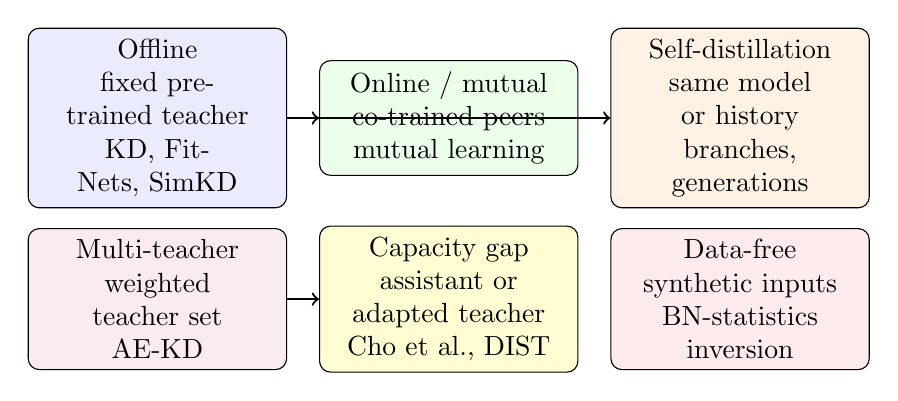
\begin{tikzpicture}[box/.style={draw,rounded corners,align=center,text width=3.0cm,minimum height=1.45cm,inner sep=4pt}, arr/.style={->,thick}]
\node[box,fill=blue!8] (offline) at (0,0) {Offline\\fixed pretrained teacher\\KD, FitNets, SimKD};
\node[box,fill=green!8] (online) at (3.7,0) {Online / mutual\\co-trained peers\\mutual learning};
\node[box,fill=orange!10] (self) at (7.4,0) {Self-distillation\\same model or history\\branches, generations};
\node[box,fill=purple!8] (multi) at (0,-2.3) {Multi-teacher\\weighted teacher set\\AE-KD};
\node[box,fill=yellow!18] (gap) at (3.7,-2.3) {Capacity gap\\assistant or adapted teacher\\Cho et al., DIST};
\node[box,fill=red!8] (free) at (7.4,-2.3) {Data-free\\synthetic inputs\\BN-statistics inversion};
\draw[arr] (offline) -- (online);
\draw[arr] (offline) -- (self);
\draw[arr] (multi) -- (gap);
\end{tikzpicture}
\caption{Training schemes differ in teacher availability, number of guidance sources, and whether original training data are available. Arrows indicate alternative arrangements, not a required progression.}
\label{fig:schemes}
\end{figure}


% Owner: Salim  |  Task: T9  |  Drafted by ORCA agents, finalised by the owner.
% Rules: prose only; every claim cited with \citet/\citep to a literature/sources.yaml record id;
% compare methods (G6); strengths/weaknesses/applicability (G8). See tasks/todo.md.
\section{Teacher Reliability and Selective Transfer}
\label{sec:reliability}
\textit{[To be written: Carried over from the original draft (L36--106); Table III.]}

% Owner: Khalid  |  Task: T10  |  Drafted by ORCA agents, finalised by the owner.
% Rules: prose only; every claim cited with \citet/\citep to a literature/sources.yaml record id;
% compare methods (G6); strengths/weaknesses/applicability (G8). See tasks/todo.md.
% Every update rule below was checked against the cited paper's PDF (2026-11-07); equation
% numbers are given in comments next to each rule.
\section{Multi-Objective Optimization: A Primer}
\label{sec:moo}

A distillation loss is almost always a sum of a supervised task loss and one or more terms that
pull the student towards the teacher. This section sets out the multi-objective optimisation (MOO)
vocabulary that \S\ref{sec:kd_moo} needs, restricted to first-order rules that pick one update
direction from per-objective gradients; \citet{chen2026gradmoo} survey the wider field.

\paragraph{Pareto optimality and stationarity.}
Consider $K$ differentiable losses $L_1,\dots,L_K$ of shared parameters $\theta$, with
gradients $g_i=\nabla_\theta L_i(\theta)$. A point $\theta^\star$ is Pareto optimal when no other
point lowers one loss without raising another; gradient methods target the local notion of
\emph{Pareto stationarity}, where some convex combination of the gradients vanishes, $\sum_i\alpha_i g_i=0$ with $\alpha_i\ge0$ and
$\sum_i\alpha_i=1$. Every Pareto optimal point is Pareto stationary but not conversely
\citep{sener2018mgda}. Away from such points a direction $d$ exists with $g_i^\top d>0$ for every
$i$, so a small step along $-d$ lowers all losses; the rules below differ in which such direction they
pick and what they do when none exists.
% sener2018mgda Sec. 3.1, KKT conditions and the remark that Pareto optimal => Pareto stationary.

\paragraph{Linear scalarisation.}
The default in distillation is the weighted sum $L=\sum_i w_iL_i$ with fixed $w_i\ge0$, whose
gradient is $\sum_i w_ig_i$, at one backward pass. As the weights vary it reaches only the convex
part of the Pareto front \citep{gong2021dbgd}, and its direction follows raw gradient norms, so a
much larger gradient dominates unless the weights are retuned. Whether this matters in practice is
contested (\S\ref{sec:kd_moo_critical}).
% gong2021dbgd Sec. 1: "(2) can only capture the convex envelop of the Pareto front".

\subsection{Symmetric rules}
\label{sec:moo_symmetric}

The first family, designed for multi-task learning, treats all objectives alike: permuting the
losses does not change the update.

\paragraph{MGDA.}
\citet{sener2018mgda} cast multi-task learning as MOO with the multiple-gradient descent
algorithm (MGDA), which picks the minimum-norm point of the convex hull of the gradients,
$\min_{\alpha\in\Delta}\|\sum_i\alpha_ig_i\|_2^2$. The result is either zero, which certifies
Pareto stationarity, or a direction that decreases every loss. For two objectives the weight
has a closed form, $\hat\alpha=\big[(g_2-g_1)^\top g_2/\|g_1-g_2\|^2\big]_{[0,1]}$; for more
objectives, Frank--Wolfe; MGDA-UB takes gradients at a shared representation to need one backward
pass. Two-objective MGDA favours the \emph{smaller} gradient (an interior minimiser has equal inner
products with both), so with a large task and a small distillation gradient it moves mostly along
distillation (Fig.~\ref{fig:moo_geometry}). It suits problems where no objective may be sacrificed,
not ones where one matters more.
% sener2018mgda Eq. (3) (min-norm problem), Eq. (4) (two-task closed form, clipped to [0,1]),
% Sec. 3.2 / Alg. 2 (Frank-Wolfe), Sec. 3.3 (MGDA-UB, gradients w.r.t. the shared representation Z).

\paragraph{PCGrad.}
\citet{yu2020pcgrad} keep each task gradient but edit it when it conflicts with another.
If $g_i^\top g_j<0$, PCGrad replaces $g_i$ by its projection onto the normal plane of $g_j$,
$g_i\leftarrow g_i-\frac{g_i^\top g_j}{\|g_j\|^2}g_j$. It repeats this for every other task in
random order and sums the results. Unlike MGDA it leaves non-conflicting gradients untouched and
keeps the scale of the sum; it needs one backward pass per objective and gives no priority, so with
two objectives the task gradient loses its distillation component as much as the reverse.
% yu2020pcgrad Alg. 1 (lines 5-8) and Sec. 2.2 projection formula.

\paragraph{CAGrad.}
\citet{liu2021cagrad} seek, within a ball around the average gradient $g_0$, the direction that
most improves the worst-off objective:
$\max_d\min_i\langle g_i,d\rangle$ subject to $\|d-g_0\|\le c\|g_0\|$. The dual is a problem over
the simplex, $\min_{w\in\Delta}g_w^\top g_0+\sqrt{\phi}\|g_w\|$ with $\phi=c^2\|g_0\|^2$, and the
update is $d=g_0+\frac{\sqrt\phi}{\|g_w\|}g_w$. With $c=0$ CAGrad is plain gradient descent on the
average loss. As $c$ grows the authors show it approaches MGDA. The radius $c$ interpolates
between the weighted sum and MGDA, and CAGrad
inherits MGDA's symmetry and per-objective backward passes, and adds one hyperparameter.
% liu2021cagrad Eq. (3) (primal), Alg. 1 (dual over the simplex and the update), Sec. 4 Q2
% (recovers GD at c = 0 and MGDA as c grows).

\paragraph{Other symmetric rules.}
Nash-MTL solves a bargaining game, $G^\top G\alpha=1/\alpha$, whose solution is invariant to
rescaling any one loss but needs an iterative solver on top of $K$ backward passes
\citep{navon2022nashmtl}; FAMO applies the MGDA problem to log-loss gradients but amortises the
weights from observed loss changes, reaching MGDA-like balancing at one backward pass with weights
that lag a step \citep{liu2023famo}; and GradNorm and uncertainty weighting only retune scalar
weights, from gradient-norm targets and learned task noise respectively, so they address scale
imbalance but not conflict \citep{chen2018gradnorm,kendall2018uncertainty}.
% navon2022nashmtl Claim 3.1 (G^T G alpha = 1/alpha), Sec. 3 (scale-invariance axiom).
% liu2023famo Prop. 3.1 / Eq. (6) (dual = min-norm on grad log losses), Sec. 3.2 (amortised O(1) update).
% chen2018gradnorm Eq. (1)-(2); kendall2018uncertainty Eq. (7).

\subsection{Priority, lexicographic and constrained rules}
\label{sec:moo_priority}

The second family drops symmetry: one objective is primary and the others are constraints, which
matches the usual reading of distillation, where the student must fit the labels and the teacher
is useful but fallible. Each rule finds the direction closest to a reference gradient subject to
linear inequalities on the others; they differ in the reference, the required progress, and the
scaling.
DBGD minimises $\|\nabla f-v\|^2$ subject to $\nabla g^\top v\ge\phi(\theta)$, with closed form
$v=\nabla f+\lambda\nabla g$ and a barrier that forces progress on $g$ until its target is met; it
has continuous-time non-convex convergence results, and the authors argue a tuned weighted sum
cannot solve the constrained problem when the duality gap is non-zero \citep{gong2021dbgd}.
GEM and A-GEM, from continual learning, project the new-task gradient so that earlier-task
gradients do not get worse, i.e.\ with zero required progress \citep{lopezpaz2017gem,chaudhry2019agem}.
PNGD stays close to an external criterion $\nabla F$ with one scheduled margin on all losses
\citep{ye2022pngd}, and AuxiNash learns a preference vector over Nash-MTL's bargaining solution, so
its priority is learned and the main task's progress is not guaranteed \citep{shamsian2023auxinash}.
% gong2021dbgd Eq. (6), Eq. (4)/Alg. 1, Eq. (8), Sec. 3.4. lopezpaz2017gem Eq. (8), (11); chaudhry2019agem Eq. (10)-(11).
% ye2022pngd Eq. (7). shamsian2023auxinash Sec. 4.1, 4.2.

\paragraph{PCD.}
Priority-constrained descent \citep{varam2026pcd} rescales each gradient by an EMA of its norm and
solves $\min_{\tilde d}\tfrac12\|\tilde d-\tilde g_1\|^2$ subject to
$\tilde g_j^\top\tilde d\ge\tau\|\tilde g_j\|^2$; for two objectives,
$\tilde d^\star=\tilde g_1+\max\big(0,\tau-\tilde g_1^\top\tilde g_2/\|\tilde g_2\|^2\big)\tilde g_2$,
rescaled to the primary gradient norm, with no correction when the constraint already holds.
The authors say the program is not new (DBGD at $K=2$; A-GEM at $\tau=0$); they add the
normalisation, which makes $\tau$ scale-free, and a general-$K$ analysis. Each secondary makes
first-order progress, but the primary is not guaranteed to descend under strong conflict, no
convergence theorem covers the deployed algorithm, and, unlike AuxiNash, the priority is fixed
rather than learned. Its evidence comes from pruning and low-rank compression, not distillation.
% varam2026pcd Def. 4.1 / Eq. (4), Def. 4.5, Cor. 4.6 / Eq. (14), Alg. 1, Sec. 4.1, Sec. 2,
% Prop. 4.4, Prop. 4.7 (primary descent only if 1 + tau c - c^2 > 0), Sec. 4.8.

\subsection{The two families side by side}

\begin{figure}[t]
\centering
\resizebox{0.6\linewidth}{!}{% Generated by paper/survey/figures/moo_geometry.py -- do not edit by hand.
% g1 = [2.0, 0.5], g2 = [-0.5, 0.8], CAGrad c = 0.5, PCD tau = 0.5
% Weighted sum: (0.7500,0.6500)
% MGDA: (0.0875,0.7295)
% PCGrad: (1.4453,1.9099)
% CAGrad: (0.4870,1.0708)
% PCD: (1.4129,1.4393)
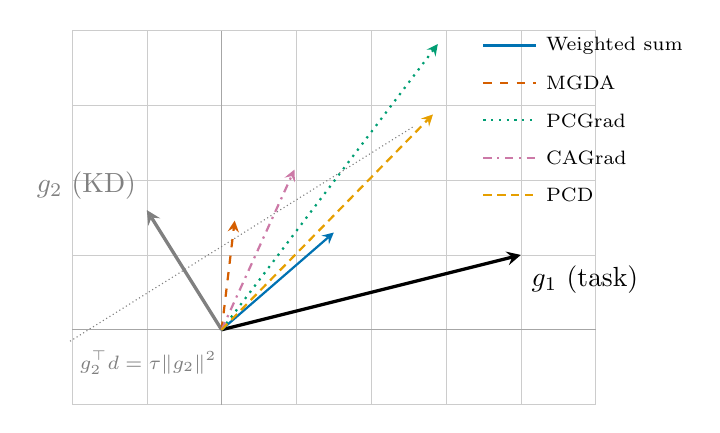
\begin{tikzpicture}[scale=1.9,>=stealth]
\draw[gray!40,very thin] (-1,-0.5) grid[step=0.5] (2.5,2);
\draw[gray!70] (-1,0) -- (2.5,0); \draw[gray!70] (0,-0.5) -- (0,2);
\draw[densely dotted,gray] (-1.0132,-0.0770) node[below right,font=\scriptsize] {$g_2^\top d=\tau\|g_2\|^2$} -- (1.2764,1.3540);
\draw[->,very thick,black] (0,0) -- (2.0000,0.5000) node[below right] {$g_1$ (task)};
\draw[->,very thick,gray] (0,0) -- (-0.5000,0.8000) node[above left] {$g_2$ (KD)};
\draw[->,thick,color={rgb,255:red,0;green,114;blue,178},solid] (0,0) -- (0.7500,0.6500);
\draw[->,thick,color={rgb,255:red,213;green,94;blue,0},dashed] (0,0) -- (0.0875,0.7295);
\draw[->,thick,color={rgb,255:red,0;green,158;blue,115},dotted] (0,0) -- (1.4453,1.9099);
\draw[->,thick,color={rgb,255:red,204;green,121;blue,167},dashdotted] (0,0) -- (0.4870,1.0708);
\draw[->,thick,color={rgb,255:red,230;green,159;blue,0},densely dashed] (0,0) -- (1.4129,1.4393);
\draw[thick,color={rgb,255:red,0;green,114;blue,178},solid] (1.75,1.90) -- (2.1,1.90) node[right,black,font=\scriptsize] {Weighted sum};
\draw[thick,color={rgb,255:red,213;green,94;blue,0},dashed] (1.75,1.65) -- (2.1,1.65) node[right,black,font=\scriptsize] {MGDA};
\draw[thick,color={rgb,255:red,0;green,158;blue,115},dotted] (1.75,1.40) -- (2.1,1.40) node[right,black,font=\scriptsize] {PCGrad};
\draw[thick,color={rgb,255:red,204;green,121;blue,167},dashdotted] (1.75,1.15) -- (2.1,1.15) node[right,black,font=\scriptsize] {CAGrad};
\draw[thick,color={rgb,255:red,230;green,159;blue,0},densely dashed] (1.75,0.90) -- (2.1,0.90) node[right,black,font=\scriptsize] {PCD};
\end{tikzpicture}
}
\caption{Directions chosen by five rules for one pair of conflicting gradients,
$g_1=(2,0.5)$ (task) and $g_2=(-0.5,0.8)$ (distillation), $g_1^\top g_2=-0.6$. Weighted sum with
equal weights; MGDA two-vector min-norm point \citep{sener2018mgda}; PCGrad
\citep{yu2020pcgrad}; CAGrad with $c=0.5$ \citep{liu2021cagrad}; PCD with $\tau=0.5$ and unit
normalisation scales, so its direction lies on the dotted line $g_2^\top d=\tau\|g_2\|^2$
\citep{varam2026pcd}. Arrows are update directions before any rescaling. The vectors are
illustrative, not measured. Generated by \texttt{figures/moo\_geometry.py}; a unit test
recomputes each direction.}
\label{fig:moo_geometry}
\end{figure}

In Fig.~\ref{fig:moo_geometry} the task gradient is about two and a half times longer than the
distillation gradient and they conflict. MGDA's direction ($83^\circ$) leans to the shorter
gradient and has almost no task component; CAGrad sits between the average and MGDA ($66^\circ$);
PCGrad returns the longest vector ($53^\circ$); PCD adds the smallest multiple of the distillation
gradient that meets its constraint ($46^\circ$), the closest to the task among the conflict-aware
rules; the equal-weight sum is closest overall ($41^\circ$) only because the task gradient is the
longer one. This does not say which rule is better: symmetric rules suit settings where every
objective must improve, priority rules settings where one objective is the reason for training.
Most conflict-aware rules need one backward pass per objective, and whether any beats a tuned
weighted sum is the empirical question of \S\ref{sec:kd_moo_critical}.
% Angles from moo_geometry.py output: WS 40.9, MGDA 83.2, PCGrad 52.9, CAGrad 65.5, PCD 45.5 degrees.

% Owner: Khalid  |  Task: T11  |  Drafted by ORCA agents, finalised by the owner.
% Rules: prose only; every claim cited with \citet/\citep to a literature/sources.yaml record id;
% compare methods (G6); strengths/weaknesses/applicability (G8). See tasks/todo.md.
\section{Knowledge Distillation as Multi-Objective Optimization}
\label{sec:kd_moo}
\textit{[To be written: How state-of-the-art KD uses MOO (AE-KD, SCKD, DOT, DTO-KD, SCOPE, TPKD, MEMA, CHAD); critical view; Table IV.]}

% Owner: Hasan  |  Task: T12, trimmed in T12c-B  |  Drafted by ORCA agents, finalised by the owner.
% Rules: prose only; every claim cited with \citet/\citep to a literature/sources.yaml record id.
% T12c-B cut the LLM, VLM, robust and federated subsections to pointers; cut citations are listed
% in the T12c-B report.
\section{Emerging Settings}
\label{sec:emerging}

\subsection{Beyond image classification}

This survey covers knowledge distillation for image classification. Several neighbouring settings reuse its ingredients but fall outside its scope. In LLM distillation the student's own generated sequences become training data, as in MiniLLM's reverse KL on student samples; UP-MOPD applies PCGrad-style projection to per-teacher updates in multi-teacher on-policy distillation, the closest LLM analogue of Section~\ref{sec:kd_moo} \citep{gu2024minillm,zhu2026upmopd}. With vision-language teachers, CLIP-KD finds simple feature mimicry a strong baseline for CLIP compression, and DHO measures CE--KD gradient conflict with a zero-shot CLIP teacher and removes it with separate heads \citep{yang2024clipkd,kang2025dho}. Adversarially robust distillation meets the reliability question of Section~\ref{sec:reliability}: a more robust teacher need not improve the student's robust generalisation \citep{lee2026robustteachers}. CA-AT projects adversarial gradients relative to clean ones in the priority style of Section~\ref{sec:kd_moo}, although its record remains an unverified preprint with a BMVC venue lead \citep{xue2024caat}. Federated distillation transfers knowledge across clients without a shared training set; DFRD performs server-side data-free distillation with a conditional generator, and FedGO weights client logits with a discriminator \citep{luo2023dfrd,jang2025fedgo}. Diffusion-model distillation is also outside the scope.
% No diffusion-model-distillation record exists in literature/sources.yaml, so no pointer is cited.

% Owner: Aly  |  Task: T13  |  Drafted by ORCA agents, finalised by the owner.
% Rules: prose only; every claim cited with \citet/\citep to a literature/sources.yaml record id;
% compare methods (G6); strengths/weaknesses/applicability (G8). See tasks/todo.md.
\section{Benchmarks and Reported Results}
\label{sec:benchmarks}
\textit{[To be written: CIFAR-100 and ImageNet tables from official sources with protocol caveats.]}

% Owner: Khalid  |  Task: T14  |  Drafted by ORCA agents, finalised by the owner.
% Rules: prose only; every claim cited with \citet/\citep to a literature/sources.yaml record id;
% compare methods (G6); strengths/weaknesses/applicability (G8). See tasks/todo.md.
\section{Open Challenges and Future Directions}
\label{sec:future}
\textit{[To be written: Gap-grounded directions (G9).]}

% Owner: Khalid  |  Task: T15  |  Drafted by ORCA agents, finalised by the owner.
% Rules: prose only; every claim cited with \citet/\citep to a literature/sources.yaml record id;
% compare methods (G6); strengths/weaknesses/applicability (G8). See tasks/todo.md.
\section{Conclusion}
\label{sec:conclusion}

This survey reviewed knowledge distillation for image classification from 2022 to 2026. Its method set was
not chosen by hand. Three searches and a gap pass over the main vision and machine-learning venues, two
journals and recent arXiv preprints produced 112 methods that meet fixed inclusion criteria, and the
exclusion of every assessed paper is recorded with a code.

The methods fall into five families. Logit methods are the largest group and the cheapest to run: they need
no projector and apply to any pair with a shared label space. Feature and relation methods give some of the
highest single-method CIFAR-100 numbers, but they need access to intermediate layers and a module per pair,
and the best of them can enlarge the deployed student \citep{chen2022simkd}. Training schemes trade accuracy
on the standard pairs for removing or reducing the cost of a fixed pre-trained teacher. Reliability methods
decide which teacher outputs to trust, or retrain the teacher for the student. A smaller group changes how the
task and distillation gradients are combined \citep{zhao2023dot,huang2025deepkd,hayder2026dtokd}. We
reviewed it next to the general multi-objective rules it borrows from, and placed priority-based rules such as
PCD \citep{varam2026pcd} among them as one option, without reported numbers on the standard pairs.

The compiled results support a cautious reading. On CIFAR-100 ResNet32$\times$4$\to$ResNet8$\times$4 the best
reported configurations are about six points above classical KD, yet most single methods lie within two
points of one another, and on ImageNet nearly all rows sit within two points. Many of the highest rows stack
one method on another, change the teacher, or add data, and the papers differ in how many runs they average.
Gaps of a few tenths of a point therefore say little. A second reading is that optimizer-side changes stack on
loss-side ones, so they should be tested on top of both plain KD and a strong logit loss.

Several questions stay open. Cross-paper comparison would improve if papers reported seed statistics and
stand-alone numbers for stacked methods. Results depend on the training recipe, as patient and consistent
teaching shows \citep{beyer2022patientkd}, and a student can generalise well while matching the teacher
poorly \citep{stanton2021kdwork}. For the objective-combination methods, the main untested point is how
often the task and distillation gradients conflict on the standard benchmarks at all, and whether the
extra gradient computations pay off when they do. The debate on whether a tuned weighted sum is enough in
multi-task learning \citep{xin2022mtohelp,kurin2022unitary,royer2023scalarization} suggests that strong
weighted-sum baselines belong in every such comparison. Section~\ref{sec:future} discusses these
directions in more detail.


\bibliography{refs}
\bibliographystyle{tmlr}

\end{document}
